% -*- root: ../main.tex -*-
\chapter{Symboliczne AI}
\label{chap:symbolic:ai}

Na poprzednich stronach rozmawialiśmy sporo o statystycznym podejściu do sztucznej inteligencji. Istnieje jednak inne podejście nazywane symbolicznym AI. Nie jest ono obecnie tak popularne czy podkreślane w nauce o sztucznej inteligencji, ale historycznie było ważną jej dziedziną. Sądzimy, że obecny ruch oddalający nas od symbolicznych pomysłów wynika częściowo z braku sukcesu w oparciu symboli o sub-symboliczne znaczenie. Ludzie, kiedy mówią o danym pojęciu, przypominają sobie wiele faktów jego dotyczących. Kiedy chociażby mówimy o kocie, to możemy mieć przed oczami jego wygląd, sposób poruszania się, wiemy, jakie jest jego ulubione jedzenie itd. Nie jest więc tak, że pojęcie kota jest niezależne od innych. Raczej należy ono do sieci pojęć, z której każde definiuje inne, z którymi jest połączone, ale jednocześnie uzyskuje swoje znaczenie poprzez inne pojęcia. Tej właściwości często brakuje w symbolicznych systemach. Są one raczej nakierowane na manipulację symbolami w sensie matematycznym. Nacisk rzadko jest położony na rozbudowywanie arsenału możliwości systemu, poprzez dodawanie nowych pojęć. Jednocześnie powiedzieliśmy, że symbole nie mają zazwyczaj połączenia z sub-symbolicznymi systemami takimi jak sieci neuronowe. Sprawia to, że symbole, którymi manipulują te systemy, nie mają dla nich takiego znaczenia jak dla nas. Jest to zupełnie inne podejście. Jednak mimo tych ograniczeń systemy manipulacji symbolami odniosły spory sukces. Podajmy tu przykład programu LT (ang. Logic Theorist) napisanego w 1956 roku przez Newell’a, Simon’a i Shaw’a. LT wykorzystywał strukturę drzewa, na której dokonywał rozumowania, aplikując zmiany do wyrażenia oparte na zasadach logiki i matematyki. Jeśli poprzez te zmiany doszedł on do rozwiązania, to kończył poszukiwania, a ścieżka prowadząca od prepozycji do wyniku była nazywana dowodem. Żeby ograniczyć rozgałęzianie możliwości, LT posiadał pewne heurystyki, które ograniczały przeprowadzanie pewnych operacji, żeby rozmiar drzewa wyszukiwań pozostawał sensowny. Program ten udowodnił 38 z 52 twierdzeń w pewnym rozdziale książki „Principia Mathematica”. Udało mu się także znaleźć bardziej elegancki dowód pewnego twierdzenia, jednak nie został on przyjęty do czasopisma matematycznego ze względu na swoją prostotę. Osoba, która oceniała to zgłoszenie, prawdopodobnie nie zauważyła, że autorem był komputer.\newline

\noindent Symboliczne systemy definiują pewien zestaw formalnych zasad i używają ich do dochodzenia do pewnych konkluzji. W ten sposób można by rozwiązać na przykład problem różniczkowania albo następujący sylogizm:

\begin{quote}
Wszyscy ludzie są śmiertelni.
\end{quote}
\begin{quote}
Sokrates jest człowiekiem.
\end{quote}

\noindent Tu chcielibyśmy, by nasz system skonkludował oczywiste:

\begin{quote}
Stąd wynika, że Sokrates jest śmiertelny.
\end{quote}

\noindent Naturalnym rozwinięciem rozumowania symbolicznego są techniki propagacji ograniczeń (ang. constraint propagation), które sprawiają, że wszystkie zdefiniowane ograniczenia są ze sobą zgodne. Na przykład możemy sprawdzić, czy następujące ograniczenia są ze sobą zgodne:

\begin{quote}
Wszystkie jabłka są czerwone.
\end{quote}
\begin{quote}
Moje jabłko jest zielone.
\end{quote}

Tu chcemy, aby nasz system skonkludował niemożliwość prawdziwości tych dwóch stwierdzeń w tym samym czasie. Na podstawie podobnych zasad działają tak zwane systemy eksperckie zawdzięczające swoją nazwę od w teorii, naśladowania eksperta. Takie systemy były początkowo najczęściej wykorzystywanymi w przemyśle. Stworzenie takiego systemu wymagało najpierw zebrania specjalistycznej wiedzy od ekspertów. Następnie zapisywało się tę wiedzę przy pomocy różnych zasad, często przy pomocy popularnych w informatyce zasad jeśli-to. Były to często metody nieróżniące się wiele od klasycznych metod programowania. Systemy eksperckie były i są wykorzystywane w różnych specjalistycznych dziedzinach np. prawie, które jest czasami podatne na sformalizowanie w taki sposób ze względu na występowanie w nim wielu zasad.\newline

Jako część metod symbolicznych uznalibyśmy także metody poszukiwania w drzewie. Te techniki dają nam sposób patrzenia na różne wybory, których moglibyśmy dokonać. Wyobraźmy, że znajdujemy się w wielkim zamku z wielkoma pokojami. Chcemy wyjść na zewnątrz, lecz nie znamy drogi, która tam prowadzi. Musimy więc spróbować drzwi, które prowadzą z naszego pokoju do innego, w którym może być wyjście. Jeśli z naszego pokoju wychodzi kilka różnych drzwi, to musimy mieć jakiś sposób dokonania wyboru pomiędzy nimi. W następnym pokoju napotkamy prawdopodobnie podobny problem, gdzie będziemy musieli wybrać między wieloma drzwiami. Metody poszukiwania w drzewie dają nam sposób na śledzenie odwiedzonych pokoi. Zbierając te informacje, dają nam one możliwość dokonywania najlepszej decyzji w danych okolicznościach.

\section{Rozwiązywanie poprzez wyszukiwanie}

Widzieliśmy już jedno rozwiązanie problemu poprzez wyszukiwanie. Czy pamiętasz, co to było? Kiedy szukaliśmy sposobu, aby znaleźć minimum funkcji wartości, zaproponowaliśmy na początku, aby sprawdzać możliwe rozwiązania w sposób losowy przez jakiś czas, a następnie wybrać najlepsze odwiedzone rozwiązanie. To jest właśnie rozwiązanie przez wyszukiwanie. Jednym z problemów, które moglibyśmy rozwiązać poprzez wyszukiwanie, jest problem \textbf{propagacji ograniczeń}. W takim problemie staramy się sprawdzić, czy wszystkie nałożone ograniczenia są ze sobą zgodne, czy mówiąc inaczej, nie zaprzeczają sobie. Na przykład w problemie kolorowania map, pytamy się, czy i w jaki sposób jesteśmy w stanie pokolorować daną mapę za pomocą $\boldsymbol{n}$ kolorów, w ten sposób, aby przylegające kraje były pokryte innymi kolorami tuszu. Dodatkowe pytanie, jakie możemy zadać to: czy istnieje, a jeśli tak to, jaka jest najmniejsza liczba kolorów, za pomocą której możemy pokolorować dowolną mapę? Na to pytanie odpowiada twierdzenie o czterech kolorach. Mówi nam ono, że za pomocą czterech kolorów jesteśmy w stanie pokolorować dowolną mapę. Taką hipotezę postawiono już w XIX w. ale na rozwiązanie tego problemu przyszło nam poczekać aż do roku 1976, w którym przy użyciu komputera sprawdzono 1936 przypadków możliwych ułożeń mapy. Jednak później powstały pewne wątpliwości co do poprawności rozwiązania, które jednak udało się rozwiać znów przy pomocy komputerowego wspomagania. Jest to jeden z ciekawszych dowodów w matematyce, ponieważ ciężko jest go sprawdzić człowiekowi i pokazuje nam, że nowy rodzaj dowodów jest możliwy. Wracając jednak do głównego tematu, przypomnijmy, że chcemy rozwiązać ten problem dla konkretnego przypadku, więc nie wystarczy nam dowód, ale potrzebujemy też konkretnych kolorów dla danych państw. Moglibyśmy w teorii rozwiązać ten problem metodą prób i błędów, ale istnieje dużo szybszy sposób. Używa on idei spójności. Kolor państwa jest spójny w węźle (ang. node-consistent), jeśli jest spójny ze samym sobą. Spójność w węźle jest w oczywisty sposób zachowana, jeśli tylko używamy legalnego koloru. Kolor będzie spójny w łuku (ang. arc-consistent), jeśli jest spójny ze samym sobą oraz z kolorami przylegających państw. Lepszym rozwiązaniem problemu kolorowania mapy jest wybranie jakiegoś koloru dla jednego państwa i sprawdzenie spójności w łuku. Następnie, jeśli rozwiązanie jest spójne, wybierzemy kolor dla innego państwa i sprawdzimy jego spójność w łuku. Postępujemy w ten sposób, tak długo aż nie rozwiązaliśmy problemu lub problem stał się niespójny. W takim przypadku cofniemy się do poprzedniego rozwiązania, które było spójne w łuku i spróbujemy innych kolorów. To cofanie nazywane jest \textbf{nawrotem} (ang. backtracking). Nawroty są dość częstym pomysłem wykorzystywanym w drzewie poszukiwań, o którym powiemy dalej. Pozwalają nam one cofnąć się do poprzednio odwiedzonego stanu i wybrać inną ścieżkę, czy to z powodu bycia niespójnym, czy też, aby sprawdzić inne możliwości. Pomysł cofania pewnych informacji w górę drzewa będzie wykorzystywany dalej w drzewach poszukiwań.

\clearpage
\begin{figure}[H]
\centering
\includepdf[pages=17]{mputo.pdf}
\caption{Propagacja ograniczeń}
\end{figure}
\clearpage

\section{Drzewa poszukiwań}

\textbf{Drzewo} jest strukturą danych, która bierze swoją nazwę z podobieństwa do drzewa. Drzewa wyrastają z korzenia, a gałęzie rozgałęziają się na coraz to mniejsze. W informatyce drzewa umieszczamy na głowie, tak że korzeń znajduje się u góry a czubek drzewa wraz z większością gałęzi na samym dole. Ten sposób rysunku sprzyja naturalnemu rozwijaniu drzew od góry do dołu, tak samo, jak podczas pisania. Drzewo jako struktura danych składa się z węzłów połączonych krawędziami. Każdy węzeł oznacza pewien stan, a krawędź istnienie pewnej relacji pomiędzy tymi stanami. Stanami może być np. numer pokoju, w którym się znajdujemy a krawędziami drzwi, które łączą te pokoje. Każdy węzeł, z którego wyrasta gałąź, nazywany jest węzłem nadrzędnym (ang. parent node), a każdy węzeł posiadający węzeł nadrzędny nazywany jest węzłem podrzędnym (ang. child node).\newline

\textbf{Drzewo poszukiwań} jest techniką, której nazwa nawiązuje do wykonywania poszukiwań na strukturze danych, jakiej jest drzewo. Opisaliśmy już jedną metaforę je opisującą, kiedy to wybierając odnogę drzewa, wybieramy kolejne drzwi. Jakiego rodzaju problemy mogłyby być dobrze opisane jako takie drzewo poszukiwań? Wygląda na to, że każdy problem, w ciągu rozwiązywania którego, wielokrotnie podejmujemy podobną decyzję, byłby podatny takiemu podejściu. Na przykład: wyszukiwanie drogi w labiryncie, planowanie diety czy granie w szachy. Wszystkie te problemy wydają się dobrze zdefiniowane dla algorytmów opierających się na drzewa. Jeśli nie rozumiesz dlaczego, to zastanówmy się nad tym problemem. Po pierwsze, aby nasze dane mogły być dobrze opisane przez drzewo, to każdy stan musi mieć ze sobą coś wspólnego, ale również każdy stan powinien być rozróżnialny od innych. I tak w labiryncie możemy zapisywać unikalne położenie, przy planowaniu diety ilość kalorii a w grze w szachy pozycję. Następnie wszystkie połączenia między stanami powinny być tego samego rodzaju. Wybieranie między naszyjnikiem a ilością kalorii nie ma większego sensu. Natomiast wybór między sałatką a burgerem jest bardziej rozsądny. Tak więc podobny rodzaj połączeń powinien występować między wszystkimi stanami, aby móc dokonać między nimi wyboru. W pewnym sensie możemy myśleć o rozgałęzianiu się drzewa, od jego korzenia, jak o różnych możliwych historiach, które się nam prezentują. Jeśli wybralibyśmy pewną odnogę drzewa i podejmowali decyzje, żeby ją osiągnąć, to ona stałaby się prawdą, a więc historią wydarzeń. Jeśli jednak podjęlibyśmy decyzje prowadzące do innego miejsca, to ono byłoby historią, która się wydarzyła. Istnieje tu pewne podobieństwo do interpretacji wielu światów w mechanice kwantowej, która mówi, że na poziomie kwantowym świat rozszczepia się na różne historie, które stają się nowymi wszechświatami. Różnica jest taka, że w mechanice kwantowej wybór jest dokonywany przez losowe zachowanie cząsteczki a w drzewach poszukiwań przez maksymalizującego cel aktora. Możemy o drzewie poszukiwań myśleć jak o wybieraniu takiego kwantowego wszechświata. Sam wybór możemy nawet zobrazować jak przechodzenie przez drzwi między kolejnymi wszechświatami. Ta metafora pomoże nam dalej w interpretacji bardziej abstrakcyjnych pomysłów związanych z drzewami poszukiwań. Wspomnieliśmy także o jednej z metod wykorzystywanych w drzewach poszukiwań, jaką jest nawrot. Pomyślmy teraz, co oznacza on w metaforze wielu światów. Jeśli odwiedzimy pewien stan i się z niego cofniemy do innego poprzedzającego stanu, to znaczy, że naprawdę go nie odwiedziliśmy. Jeśli rzeczywiście byśmy w nim byli to znaczy, że nie moglibyśmy się cofnąć do poprzedzającego stanu, ponieważ czas płynie tylko w jedną stronę. Jednak w nawrocie cofamy się do poprzedzającego stanu. Oznacza to, że nie byliśmy w tym stanie, a więc było to tylko nasze wyobrażenie bycia w danym stanie. Inaczej mówiąc, przeprowadziliśmy symulację. Symulacje są jednym z ulubionych narzędzi w skrzynce kogoś zajmującego się sztuczną inteligencją. Co oznacza słowo symulacja? Symulacja jest pewnym uproszczeniem rzeczywistości, które jednak zachowuje pewne ważne jego elementy w celu przewidywania przyszłości. Próbujemy symulować zachowania, żeby podejmować najlepsze decyzje. Ludzie tworzą przeróżne symulacje, zaczynając od ekonomicznych i finansowych, symulacji zachowania ludzi i tłumów, symulacje działania pojazdów, symulacje robotów. Ludzie programujący rozwiązania sztucznej inteligencji lubią symulacje, ponieważ pozwalają im one na sprawdzanie swoich systemów w środowisku testowym. Symulowana rzeczywistość może nam też dostarczyć danych do trenowania naszych systemów takich jak sieci neuronowe. Dużo ciężej jest wpuścić system sztucznej inteligencji do prawdziwego świata niż do symulacji, co wynika z zagrożeń z tym związanych, możliwości testowania systemu, jak już wcześniej wspomnieliśmy, i sposobów komunikacji takiego aktora z rzeczywistością. Czasami, żeby działać w rzeczywistości, konieczny byłby robot, w przeciwieństwie do symulacji. Dlatego właśnie naukowcy wolą zazwyczaj używać do badań środowisk testowych, jakimi są symulacje. Najprostsze takie modele rzeczywistości powstały dawno temu na bliskim wschodzie i gdzieś w Azji. Mowa tu oczywiście o grach planszowych takich jak szachy, Go, shogi. Oddają one pewien aspekt rzeczywistości w uproszczonej formie. Chociażby szachy były symulacją kierowania polem walki. Takie proste gry są nam dzisiaj bardzo przydatne do rozwijania rozwiązań sztucznej inteligencji. Właśnie na nich z sukcesem zastosowano techniki drzew poszukiwań, i to one stoją za niektórymi najnowszymi postępami w dziedzinie, służąc jako środowisko testowe.

\clearpage
\begin{figure}[H]
\centering
\includepdf[pages=13]{mputo.pdf}
\caption{Drzewo poszukiwań}
\end{figure}
\clearpage

\section{Poszukiwanie na głębokość i rozpiętość}

Powinniśmy teraz skupić się na problemie kolejności, w której będziemy sprawdzać możliwe przyszłości. Możemy o tym myśleć jak o planie jak otwierać kolejne drzwi. Zastanówmy się jakie podstawowe właściwości ma drzewo poszukiwań. Patrząc się, nawet wizualnie, możemy wyróżnić dwie główne cechy węzłów w drzewie. Jak myślisz jakie są to cechy? Jednymi z ważniejszych cech jest to, jak głęboko węzeł znajduje się względem korzenia i ilość rozgałęzień, na które się rozgałęzia. Na tych dwóch cechach skupiają się algorytmy poszukiwania na głębokość i na rozpiętość. Jednym sposobem na eksplorowanie takiego drzewa poszukiwań jest patrzeć się tak głęboko, jak to jest możliwe, nie zwracając uwagi na inne drogi, które moglibyśmy obrać. To podejście ma nazwę \textbf{poszukiwania w głąb} (ang. depth first). Algorytm poszukiwania w głąb zawsze na początku będzie się starał patrzeć, jak najgłębiej jest to możliwe, wybierając do sprawdzenia w następnej kolejności zawsze węzeł podrzędny, jeśli jest to możliwe. Kiedy osiągamy węzeł końcowy, musimy się nawrócić do ostatniego miejsca, w którym mieliśmy wybór i stamtąd rozpocząć nasze poszukiwania, w podobny sposób, nie odwiedzając już jednak raz odwiedzonych węzłów, jeśli nie jest to konieczne. Jeśli wrócimy do naszej metafory o wybieraniu drzwi w zamku, odpowiadałoby to wybieranie pierwszych napotkanych drzwi w pokoju i przechodzenie dalej do momentu aż znajdziemy wyjście albo napotkamy na pokój bez drzwi. Kiedy dojdziemy do takiego pokoju, to zawracamy do poprzedniego pokoju, w którym byliśmy i kontynuujemy poszukiwania w ten sam sposób. Jakie mocne strony ma ten algorytm? Jedną silną stroną tego podejścia jest to, że nie musimy być bardzo dobrzy w ocenianiu sytuacji, w której jesteśmy, ponieważ dostajemy się do logicznego końca możliwości i to tam możemy dokonać oceny. Jedną słabą stroną poszukiwania w głąb jest to, że nie sprawdza ono wielu możliwości, tylko ślepo wybiera jedną drogę, którą podąża. Zupełnie inną możliwością jest \textbf{poszukiwanie wszerz}. Analogicznie do poszukiwania w głąb, poszukiwanie wszerz będzie najpierw sprawdzać wszystkie możliwości na jednym poziomie, zanim będzie poruszać się w głąb. Zużywa ono wszystkie węzły podrzędne przed przejściem do węzłów podrzędnych względem podrzędnych. W naszej metaforze zamku musimy najpierw sprawdzić wszystkie drzwi prowadzące z naszego pokoju, później sprawdzamy wszystkie drzwi w pokojach, do których prowadzą drzwi z naszego pokoju itd. Żeby to wszystko ogarnąć, musielibyśmy stworzyć mapę i zapisywać na niej wszystkie połączenia. Podobnie działają oba z tych algorytmów. Zapisują odwiedzone stany w strukturze drzewa. Silne i słabe strony algorytmu poszukiwania wszerz będą zamienione z poszukiwaniem w głąb. To podejście bierze pod uwagę wszystkie możliwe wybory przed przejściem w głąb, a więc sprawdza wszystkie możliwości, które napotyka. Wiąże się to jednak, z tym że może nie dojść tak głęboko, jak poszukiwanie w głąb, jeśli nie otrzyma wystarczającego czasu, więc system oceniający sytuację musi być dobry, ponieważ tylko kilka ruchów w głąb, gdzie będzie trzeba dokonać wyboru, może być niejasnym czy sytuacja jest korzystna. Obie te metody mimo swoich różnic są w pewien sposób do siebie podobne. Stanowią, jak można by powiedzieć, swoje lustrzane odbicie. Są jednymi z najprostszych metod przeszukiwania drzewa. Obrazują jednocześnie kluczowy problem, który napotykamy podczas wyboru następnego węzła, który chcemy odwiedzić. Czy należy sprawdzić wiele alternatyw, czy lepiej poruszać się głębiej? Ten problem będzie dla nas dalej istotny i algorytmy dalej zaprezentowane mają unikalne metody radzenia sobie z nimi. Obie z tych metod utrzymują również w pamięci najlepszy do tej pory odwiedzony węzeł, aby zwrócić go jako odpowiedź. Kiedy odwiedzamy nowy węzeł, zawsze sprawdzamy, czy nie jest lepszy od do tej pory najlepszego i jeśli tak to zamieniamy najlepszy węzeł na obecnie odwiedzany. Ta właściwość wymaga funkcji wartości, która będzie w stanie ocenić każdy odwiedzony stan. W algorytmach tu zaprezentowanych funkcja wartości jest używana dopiero na końcu po fazie rozwijania węzłów. Węzły są najpierw rozwijane, a następnie ocena przez funkcję wartości jest stosowana na węzłach liściach, czyli takich, które nie mają żadnych podrzędnych węzłów. Spośród węzłów liści wybierana jest najlepsza gałąź, a następnie cofamy się do początku tej gałęzi i dokonujemy pierwszego wyboru, który prowadzi do tej najkorzystniejszej historii. W następnym ruchu zazwyczaj wszystko jest resetowane i poszukiwanie rozpoczyna się na nowo. Ważne jest tu także to, że sposób symulacji następnych stanów musi być dobry przy dużej ilości rozgałęzień, tak żeby ocena sytuacji w węźle liściu nie odbiegała zbyt dużo od poprawnej oceny naszej sytuacji z powodu różnic między zasymulowanym a prawdziwym rozwinięciem. Dlatego tego typu algorytmy nadają się najlepiej do sytuacji, w których symulacja jest idealna takich jak np. szachy. W szachach możemy dokładnie powiedzieć jakie możliwości istnieją w danej sytuacji i do czego prowadzą, dlatego będziemy dalej wykorzystywać ten przykład.

\clearpage
\begin{figure}[H]
\centering
\includepdf[pages=15]{mputo.pdf}
\caption{Poszukiwanie na rozpiętość i głębokość}
\end{figure}
\clearpage



\section{Minimax}

Mówiliśmy o tym, że możemy próbować rozwiązać gry dla dwóch graczy, takie jak warcaby czy szachy używając technik wyszukiwania. Czy to znaczy, że możemy po prostu wziąć algorytm poszukiwania w głąb lub wszerz i wykorzystać go do znalezienia najlepszego ruchu? Używając tamtych algorytmów, musieliśmy podać funkcję wartości i wybieraliśmy ruch ze względu na jej maksymalizację, ale na przykład w szachach, ta sama pozycja może mieć zupełne inną wartość, w zależności od tego, czyj ruch jest następny. Tak dzieje się, ponieważ jeden z graczy chce maksymalizować a drugi minimalizować tę samą funkcję wartości. Załóżmy, że wygrana białego to +1 a wygrana czarnego to -1, remis oznaczmy jako 0. W takiej sytuacji biały chce, żeby funkcja wartości była jak najbliżej 1, bo to daje mu największe szanse na wygraną, natomiast czarny przeciwnie, chce żeby funkcja wartości była jak najniższa i znajdowała się jak najbliżej -1.\newline

\begin{equation}
v_{hat} = max[min[v(a_a, a_b)]]
\end{equation}

\noindent Gdzie $\boldsymbol{v_{hat}}$ oznacza funkcję wartości dla jednego z graczy po ruchu przeciwnika i własnym, $\boldsymbol{v}$ oznacza funkcję wartości z jednej perspektywy w zależności od ruchów $\boldsymbol{a_a}$ własnym i $\boldsymbol{a_b}$ oponenta.\newline

Widzimy, że zachodzi tu rekursywna zależność, gdzie jeden z graczy chce minimalizować funkcję a drugi ją maksymalizować, i tak przy każdym ruchu. Nie możemy więc patrzeć tylko na nasze własne ruchy, bo przeciwnik będzie się starał znaleźć luki w naszym rozumowaniu. Musimy patrzeć się na przemian na ruchy dla nas i dla naszego rywala. Chociaż chcemy wybrać najlepszy ruch, to musimy go wybrać z perspektywy najgorszej możliwej sytuacji, którą wybierze dla nas nasz przeciwnik. Jednakże on ma ten sam problem, musi wybrać najgorszy ruch dla nas, wybierając wśród najlepszych ruchów, które zrobimy i tak dalej.

\clearpage
\begin{figure}[H]
\centering
\includepdf[pages=18]{mputo.pdf}
\caption{Minimax}
\end{figure}
\clearpage

\begin{equation}
v_{hat} = max[min[max[min[…]]]]
\end{equation}

Możemy zobaczyć, że występuje tu rekursywność, w której etap maksymalizacji następuje po etapie minimalizacji, a po etapie minimalizacji następuje etap maksymalizacji itd. Ta seria wydarzeń prowadzi nas bezpośrednio do pomysłu na algorytm, który wykorzystuje tę zależność. Ten algorytm patrzący się kolejno i próbujący maksymalizować funkcję wartości dla jednego poziomu węzłów i minimalizować dla kolejnego nazywa się \textbf{minimax}. Powtórzmy jeszcze raz, jak wygląda jego działanie na przykładzie szachów. Kiedy następuje nasza tura, najpierw określamy wszystkie ruchy, które możemy wykonać i zapisujemy je w drzewie, następnie przechodzimy do powstałych sytuacji i robimy to samo tym razem dla ruchów przeciwnika. Kiedy dojdziemy do pozycji końcowej, np. 'mata' to określamy, kto wygrał i zaprzestajemy poszukiwania. Jednak prawie nigdy nie korzysta się w rzeczywistości z wyszukiwania do końca ze względu na astronomicznie rosnącą liczbę rozgałęzień. Na ogół w pewnym momencie musimy przerwać poszukiwanie i określić wartość niedokończonej sytuacji w węźle za pomocą chociażby sieci neuronowej. Kiedy określimy która gałąź jest najkorzystniejsza, to wybieramy ją i cofamy się do pierwszego ruchu w tej sekwencji. Wykonujemy znaleziony ruch. Czasami w algorytmie minimax nastąpi sytuacja, w której inna gałąź jest wybrana ponad gałąź, którą eksplorujemy i zobaczenie jakiejkolwiek nowej wartości, jakkolwiek dobrej dla nas, nie zmieni ruch, który wykona nasz przeciwnik. Właściwie im lepszą możliwość znajdziemy, tym bardziej przeciwnik nie będzie chciał tam iść w ruchu poprzedzającym, tak więc znalezienie lepszej dla nas sytuacji, gdy jesteśmy przekonani, że przeciwnik i tak nie wybierze tego rozgałęzienia, ze względu na to, że nie jest dla niego dobre jeszce przed sprawdzeniem nowego rozgałęzienia, nie ma sensu. W takiej sytuacji możliwym jest, aby dokonać płytkiego lub głębokiego odcięcia gałęzi, to znaczy, że nie będziemy takiej gałęzi więcej przeszukiwać. Ta technika nazywana jest odcięciem \textbf{alfa-beta} (ang. alpha-beta pruning) i jest często używanym dodatkiem do techniki minimax. Powinna ona być właściwie używana zawsze, gdy mamy taką możliwość, ponieważ ucina ona tylko gałęzie, które nie mogą mieć wpływu na wynik wyszukiwania. Tak więc wyszukiwanie alfa-beta jest równoważne w wyniku do wyszukiwania minimax.\newline

Deep Blue, które pokonało Kasparova w słynnej serii meczów, używało algorytmu alfa-beta, który działał w paraleliźmie na wielu specjalnie do tego przygotowanych procesorach, używał skonstruowanej na te potrzeby funkcji ewaluacji, której parametry były nauczone przez system. Co ciekawe Deep Blue korzystało z wersji algorytmu zwanej \textbf{iteracyjne pogłębianie} (ang. iterative deepening) co oznacza, że wyszukiwanie jest ograniczone do pewnego poziomu głębokości i po jego osiągnięciu najlepszy do tej pory wynik zostaje zwrócony, natomiast jeśli pozostało jeszcze czasu na obliczenia, to wybierany jest pewien głębszy poziom graniczny, do którego prowadzi się poszukiwanie. Ten proces powtarzany jest wielokrotnie w ciągu wyszukiwania jednego ruchu i najlepszy ruch jest zmieniany na ten osiągnięty najgłębszym do tej pory wyszukiwaniem w miarę zwiększania głębokości. Trzeba zauważyć, że rezultaty poprzedniego wyszukiwania zostają utracone w kolejnym wyszukiwaniu, które prowadzi się od nowa. Może ci się to wydawać dużym marnotrawstwem, ale należy pamiętać, że głębsze poziomy zawierają eksponencjalne więcej węzłów niż te bliżej korzenia, więc straty osiągane przy każdym wyszukiwaniu maleją eksponencjalne w porównaniu do wyszukiwania z maksymalnym poziomem głębokości. Co daje nam ten algorytm? Zauważyliśmy, że w czasie jednego wyszukiwania kilka ruchów będzie zwróconych. Teraz, jeśli okazuje się, że nie wiemy dokładnie, ile ma trwać wyszukiwanie, to dzięki tej metodzie będziemy mieć gotowy dobry rezultat w trakcie całego trwania wyszukiwania.



\section{A*}

A* (czytaj z ang. A star) jest algorytmem \textbf{najpierw najlepsze} (ang. best first) co znaczy, że wyszukuje na początku te węzły, które podejrzewa, że będą najlepsze. Żeby to zrobić, potrzebuje pewnego sposobu estymacji funkcji wartości. Gałęzią sprawdzaną przez A* będzie ta, która minimalizuje koszt dotarcia do węzła i spodziewany koszt od tego węzła.

\begin{equation}
min[v(n)] = min[g(n) + h(n)]
\end{equation}

Gdzie $\boldsymbol{v}$ jest funkcją wartości, $\boldsymbol{g}$ jest kosztem dotarcia do węzła, a $\boldsymbol{h}$ jest spodziewanym kosztem od tego węzła do celu.\newline

Najprostszym przykładem sytuacji, w której A* byłby użyteczny, jest problem poszukiwania najlepszej ścieżki. Powiedzmy na przykład, że chcemy znaleźć drogę prowadzącą z miasta A do miasta B, która prowadzi przez pewien zbiór miast C. Może poruszamy się z miasta A do B często, więc chcemy znaleźć najlepszą ścieżkę, która prowadzi z A do B. Nie znamy jednak dokładnych odległości między miastami. W tym przypadku możemy użyć algorytmu A*, gdzie $\boldsymbol{g}$ byłoby realnym czasem drogi, którą pokonaliśmy przeliczonym na dystans, a $\boldsymbol{h}$ odległością pomiędzy miastami na mapie, spośród których próbujemy wybrać najkorzystniejsze. Widzimy więc, że część funkcji wartości zależy od rzeczywiście przebytego dystansu, a druga część od spodziewanego dystansu do przebycia. Naprawdę niekoniecznie musi to być dystans przebyty, a mogą być to wielkości na mapie. Kiedy np. program próbuje znaleźć najlepszą trasę dla naszego samochodu, wykorzystuje rozwiązania podobne do algorytmu A*. Sprawdza, ile wynosi odległość w linii prostej do celu w kilku punktach, do których możemy pojechać i dodaje do niej odległość rzeczywistej drogi prowadzącej do tych punktów, która jest do pokonania. Następnie przesuwa się do tych punktów i wykonuje podobną procedurę aż do znalezienia najlepszej trasy. Algorytm A* ma tę korzystną właściwość, że odległość spodziewana $\boldsymbol{h}$ jest zawsze mniejsza niż rzeczywista odległość, którą pokonamy. Pozwala to na określenie właściwości, która mówi, że koszt dotarcia do sąsiedniego następującego węzła i podróż od niego do celu jest zawsze nie większa niż bezpośredni koszt podróży do celu z naszego węzła. Może się to wydawać oczywiste, ale nie musi być zawsze zapewnione dla generalnego przypadku wyszukiwania na grafie. Algorytm A* został po raz pierwszy użyty w robocie Shakey, który był robotem poruszającym się samodzielnie na kołach pomiędzy pewnymi miejscami. Potrzebował więc sposobu planowania swojej trasy. Shakey miał dostawać zadanie i być w stanie rozbić je na mniejsze części, które będą konieczne do realizacji celu. Shakey do realizowania tego celu posiadał kilka umiejętności. Potrafił podróżować z jednej lokacji do drugiej (dzięki algorytmowi A*), otwierać drzwi, włączać światła, popychać obiekty. Robot posiadał system wizji, dzięki któremu orientował się w otoczeniu. Te umiejętności pozwalały mu na wykonywanie prostych zadań. Shakey był jednym z pierwszych projektów integrujących robotykę i AI, używając wiedzy z obu dziedzin do stworzenia autonomicznego robota.

\section{MCTS}

\textbf{Drzewo poszukiwań Monte Carlo} (ang. Monte Carlo tree search) w skórcie MCTS, jest metodą, którą polega w mocny sposób na losowości, stąd Monte Carlo w nazwie. MCTS nie potrzebuje funkcji wartości, ponieważ dokonuje tzw. \textbf{rozwinięć} (ang. rollout) co oznacza, że zostaje przeprowadzona symulacja od liścia do węzła końcowego, czyli takiego, który nie ma żadnych węzłów podrzędnych. Symulacja odbywa się poprzez wybranie losowej akcji i użycie jej i modelu świata do wygenerowania następnej sytuacji. Powtarzamy tę czynność, aż nie dojdziemy do węzła końcowego. W tym przypadku musimy co prawda użyć funkcji wartości do określenia sytuacji końcowej i nawrócenia wartości do liścia, jednak w grach, w których ten algorytm jest często stosowany jest inaczej. Na końcu rozgrywki funkcja wartości jest powszechnie znana, ponieważ jest to rezultat gry, a on musi być jasno określony w zasadach. Nie musimy wiedzieć nic więcej poza zasadami takiej gry. Tak więc np. w przypadku szachów dokonujemy najpierw losowego posunięcia dla nas, powiedzmy, poruszamy skoczkiem, następnie wykonujemy posunięcie dla przeciwnika, powiedzmy, ruszamy pionkiem. Kontynuujemy tak na przemian, aż nie dojdziemy przypadkowo do sytuacji, w której gra jest matem, patem lub remisem. Wtedy określamy wartość dla danego węzła końcowego. Dla szachów może to być +1, 0 lub -1. Każdy węzeł utrzymuje informacje o dwóch zmiennych, sumie wartości węzłów podrzędnych $\boldsymbol{v}$ oraz liczbie wizyt węzła $\boldsymbol{n}$. Kiedy rozwinięcie jest przeprowadzane to wartości $\boldsymbol{v}$ i $\boldsymbol{n}$ są nawracane do węzłów nadrzędnych, a stamtąd do węzłów nadrzędnych do tych nadrzędnych itd. Na każdym nadrzędnym poziomie wartości $\boldsymbol{v}$ i $\boldsymbol{n}$ są zmieniane poprzez dodanie następujących wartości:

\clearpage
\begin{figure}[H]
\centering
\includepdf[pages=14]{mputo.pdf}
\caption{MCTS}
\end{figure}
\clearpage

\begin{equation}
\delta_v = \text{value of rollout}
\end{equation}
\begin{equation}
\delta_n = 1
\end{equation}

\noindent Gdzie $\boldsymbol{v}$ zmienia się o wartość rozwinięcia, a $\boldsymbol{n}$ jest zwiększane o 1, co znaczy, że jedna dodatkowa symulacja została przeprowadzona.\newline

Kiedy rozwinięcie zostaje przeprowadzone to cała ścieżka, która nas do tego miejsca doprowadziła, zostaje wykasowana z pamięci, a pozostają jedynie informacje o $\boldsymbol{\delta_v}$ i $\boldsymbol{\delta_n}$. Te informacje są używane do odpowiedniej zmiany wartości węzłów nadrzędnych. Na razie nie powiedzieliśmy, skąd te węzły się biorą i pozostawimy tę informację na koniec. Teraz musisz jedynie wiedzieć, że tak jak w innych algorytmach poszukiwania te węzły istnieją i są czymś innym niż rozwinięcie. Rozwinięcie jest jedynie swego rodzaju próbkowaniem rzeczywistości. Wszystko, co jest konieczne do takiego próbkowania, zostaje usunięte z pamięci, a zostają pozostawione tylko węzły, z których przeprowadzamy to próbkowanie. Żeby wybrać kolejny węzeł, z którego chcemy przeprowadzić rozwinięcie, potrzebujemy jakiegoś równania, które określi nam wartość rozwinięcia z danego węzła. Co możemy zawrzeć w takim równaniu? Po pierwsze chcielibyśmy, aby częściej wizytowane były węzły, które są lepsze, czyli mają większą wartość $\boldsymbol{v}$, ponieważ chcemy sprawdzić czy są rzeczywiście tak dobre jak to ustaliliśmy. Musimy jednak pamiętać, że $\boldsymbol{v}$ będzie zależeć od wartości $\boldsymbol{n}$ czyli ilości takich rozwinięć. Tak więc dobrze byłoby, gdyby to równanie zależało od $\boldsymbol{v/n}$. Taka jest też pierwsza część równania. Jeśli jednak zawarlibyśmy tylko te informacje, to ‘dobre’ węzły byłyby jedynymi odwiedzanymi. Może się jednak zdarzyć tak, że jedna symulacja, jedno rozwinięcie jest złe, ale wszystkie inne wypadłyby dobrze. Z funkcją wybierającą węzły $\boldsymbol{v/n}$ do rozwinięcia nie jest możliwe, żeby sprawdzić węzeł, któremu się nie poszczęściło. Tak więc dodana jest druga część tego równania, która zależy od ilości odwiedzin $\boldsymbol{n}$ w stosunku do wszystkich przeprowadzonych rozwinięć $\boldsymbol{N}$. Druga część równania ma formę: $\sqrt{( ln(N) / n)}$. Ta druga część równania odpowiada za pewność na temat wielkości $\boldsymbol{v}$, im więcej próbkowań, tym bardziej jest ona pewna. Całe równanie zaś przedstawia się następująco:

\begin{equation}
 UCB1 = v/n + c * \sqrt{( ln(N) / n)}
\end{equation}

\noindent Żeby wybrać kolejny węzeł, w którym chcemy przeprowadzić rozwinięcie, musimy znaleźć węzeł z największą wartością UCT, która może być równa np. UCB1. Tu $\boldsymbol{v}$ i $\boldsymbol{n}$ są wartością węzła i ilością rozwinięć z węzła, $\boldsymbol{c}$ jest stałą wymiany pomiędzy pierwszym a drugim wyrażeniem, a $\boldsymbol{N}$ jest liczbą wszystkich przeprowadzonych symulacji w całym drzewie. UCB1 sprawia, że odwiedzane są te węzły posiadające najwyższą wartość oraz te, które były rzadko odwiedzane.\newline

Pozostała nam ostatnia rzecz: jeśli napotykamy na węzeł, którego $\boldsymbol{n}$ jest większe od zera, to znaczy jakieś rozwinięcie było poprzednio wykonane z tego węzła, wtedy rozwijamy węzeł o wszystkie akcje, które możemy wykonać. Np. w przykładzie szachowym tworzymy węzły podrzędne zawierające wszystkie posunięcia konikiem, pionkiem, wieżą itd. Jest to proces dokładnie taki sam jak w poprzednich algorytmach, tylko że dla jednego poziomu. Następnie wybieramy węzeł z największym UCT, w tym wypadku UCT są jednak równe, bo n = 0 więc UCB1 = inf., tak więc pozostaje nam wybrać węzeł spośród węzłów podrzędnych zgodnie z kolejnością alfabetyczną. Z tego węzła przeprowadzamy kolejne rozwinięcie. Ostatecznie po przeprowadzeniu wielu rozwinięć, żeby wybrać ruch, wybieramy spośród węzłów podrzędnych do korzenia, czyli naszego początkowego węzła. Wybieramy ten węzeł z największą wartością rozwinięć $\boldsymbol{n}$, ale tylko dla węzłów bezpośrednio podrzędnych. Poszukiwanie Monte Carlo wraz ze wzrastającą liczbą rozwinięć zbiega się do optymalnego rozwiązania.


